\documentclass[tikz,border=5mm]{standalone}
\usetikzlibrary{shapes.geometric, arrows.meta, positioning, fit, backgrounds, calc}
\begin{document}
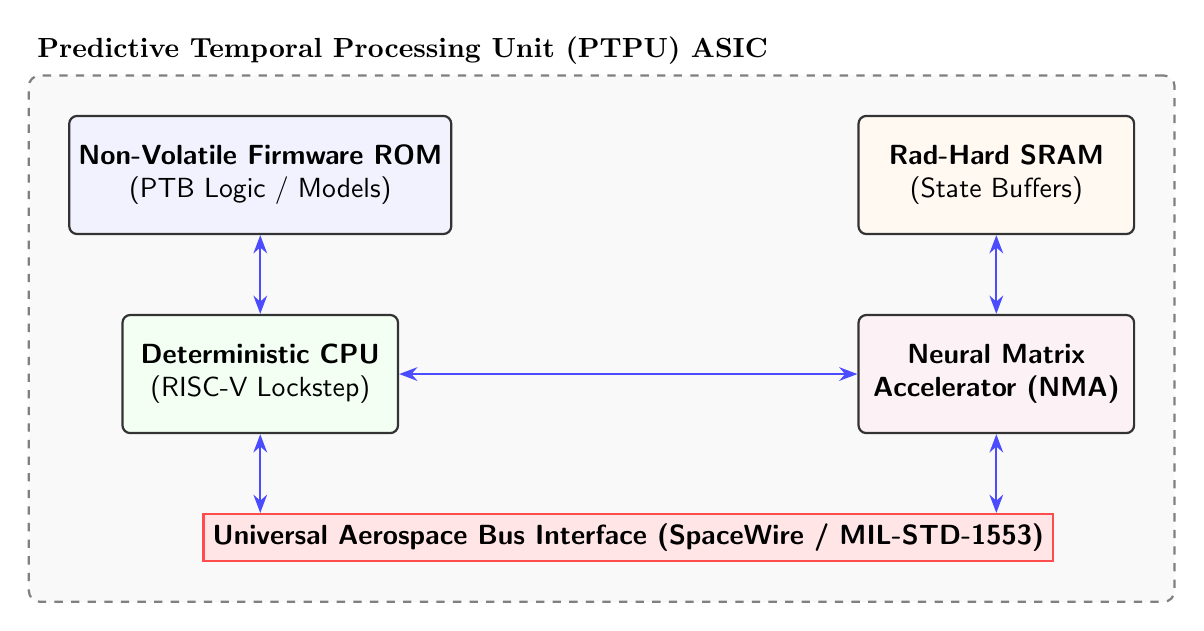
\begin{tikzpicture}[
    font=\sffamily,
    box/.style={rectangle, draw=black!80, fill=white, thick, rounded corners=1mm, minimum width=3.5cm, minimum height=1.5cm, align=center},
    bus/.style={rectangle, draw=red!70, fill=red!10, thick, minimum width=9cm, minimum height=0.6cm, align=center},
    arrow/.style={<->, >=Stealth, thick, draw=blue!70}
]

\node[bus] (bus) {\textbf{Universal Aerospace Bus Interface (SpaceWire / MIL-STD-1553)}};

\node[box, fill=green!5, above left=1cm and -2.5cm of bus] (cpu) {\textbf{Deterministic CPU}\\(RISC-V Lockstep)};
\node[box, fill=purple!5, above right=1cm and -2.5cm of bus] (nma) {\textbf{Neural Matrix}\\ \textbf{Accelerator (NMA)}};
\node[box, fill=blue!5, above=1cm of cpu] (rom) {\textbf{Non-Volatile Firmware ROM}\\(PTB Logic / Models)};
\node[box, fill=orange!5, above=1cm of nma] (sram) {\textbf{Rad-Hard SRAM}\\(State Buffers)};

\draw[arrow] (cpu.south) -- (cpu.south |- bus.north);
\draw[arrow] (nma.south) -- (nma.south |- bus.north);
\draw[arrow] (rom.south) -- (cpu.north);
\draw[arrow] (sram.south) -- (nma.north);
\draw[arrow] (cpu.east) -- (nma.west);

\begin{scope}[on background layer]
    \node[rectangle, draw=gray, dashed, thick, rounded corners, fit=(bus)(cpu)(nma)(rom)(sram), inner sep=5mm, fill=gray!5] (chip) {};
    \node[anchor=south west, font=\bfseries] at (chip.north west) {Predictive Temporal Processing Unit (PTPU) ASIC};
\end{scope}

\end{tikzpicture}
\end{document}
